\documentclass[12pt,phd,times]{pkmthesis}
\usepackage{amsmath,epsfig,graphicx,setspace,url,float}
\usepackage{pstricks,colortab,pifont}
\usepackage{lscape,multicol,multirow,longtable,subfigure}
\usepackage{cite, bm}                           % Due to this hyberref will not work for references (PKM on 07/07/08)
\usepackage[english]{babel}
\usepackage[small,bf]{caption}              % Added on 26/08/08
\captionsetup[table]{position=top}          % table captions sit above the table
%\usepackage{slashbox}
\usepackage{csquotes}
\usepackage{threeparttable}
%\usepackage{adjustbox}                    % Added on 24/10/08 (Senthil)
\setlength{\textfloatsep}{1cm}              % Spacing b/w  float and text (PKM 01/11/08)
%..........................................................................................................................................
\normalem                                   % Added on 01/07/08 to avoid underline in the references
\setlength{\abovecaptionskip}{8pt}          % Added on 08/07/08
\setlength{\belowcaptionskip}{8pt}          % Added on 08/07/08
%..........................................................................................................................................
% ---- Packages added for this report (diagrams, tables, algorithm box) ----
\usepackage[table]{xcolor}
\usepackage{tikz}
\usetikzlibrary{arrows.meta,positioning,fit,calc,shapes.geometric,backgrounds}
\tikzset{every picture/.append style={execute at begin picture={\linespread{1}\selectfont}}} % single-spaced text inside diagrams
\usepackage{array,tabularx,makecell}
\usepackage{algorithm}
\usepackage{algpseudocode}
\newcolumntype{L}[1]{>{\raggedright\arraybackslash}p{#1}}
\newcolumntype{C}[1]{>{\centering\arraybackslash}p{#1}}
\graphicspath{{figures/basepaper/}{figures/replication/}}
% ---- Custom macros used in the text ----
\newcommand{\GPN}{\textsc{GPN}}
\newcommand{\eps}{\varepsilon}
%..........................................................................................................................................
\usepackage{hyperref}
\usepackage{extra_functions}
%%*************************************************  MARGINS  ************************************************
% FOR SINGLE SIDE
%\hoffset 0in
%\voffset 0in
%\oddsidemargin 0.40cm
%\evensidemargin 0.55cm
%\marginparsep 0in
%\topmargin -0.25cm
%\textwidth 17cm
%\textheight 23.5cm
%\footskip 1.5cm

% FOR DOUBLE SIDE (03/09/08)
\hoffset 0in
\voffset 0in
\evensidemargin -0.4in
\oddsidemargin
 0.2cm
 \marginparsep 0in
 \topmargin 0.25cm
 \textwidth 17cm
\textheight 22.5cm
\footskip 1.5cm


%*************************************************************************************************************

\usepackage{fancyhdr}
\pagestyle{fancy}

%*************************************************************************************************************

\renewcommand{\chaptermark}[1]{\markboth{\thechapter.\ #1}{}}
\renewcommand{\sectionmark}[1]{\markright{\thesection\ #1}}

%\fancyhf{} \fancyhead[LE]{\bfseries\nouppercase{\leftmark}}
%\fancyhead[RO]{\bfseries\nouppercase{\rightmark}}

%*************************************************************************************************************
% HEADER & FOOTER HEADINGS  %PKM 04/07/08
%*************************************************************************************************************

\renewcommand{\headrulewidth}{0.5pt}
\renewcommand{\footrulewidth}{0.5pt}
\addtolength{\headheight}{2pt} % make space for the rule

%*************************************************************************************************************

\fancypagestyle{plain}{%
   \fancyhead{} % get rid of headers
   \renewcommand{\headrulewidth}{0pt} % and the line
   \renewcommand{\footrulewidth}{0pt}
}

%*************************************************************************************************************

\fancypagestyle{blank}{%
   \fancyhf{} % get rid of headers and footers
   \renewcommand{\headrulewidth}{0pt} % and the line
   \renewcommand{\footrulewidth}{0pt}
}

%*************************************************************************************************************

\fancypagestyle{abstract}{%
   \fancyhead{}
   \renewcommand{\headrulewidth}{0pt}
   \renewcommand{\footrulewidth}{0.5pt}
}

%*************************************************************************************************************

\fancypagestyle{document}{%
    \fancyhf{} \fancyhead[LE]{\bfseries\nouppercase{\leftmark}}
    \fancyhead[RO]{\bfseries\nouppercase{\rightmark}}
    \fancyfoot[LE,RO]{\bfseries\thepage}
    \renewcommand{\headrulewidth}{0.5pt}
    \renewcommand{\footrulewidth}{0.5pt}
    \addtolength{\headheight}{2pt} % make space for the rule
}

%*************************************************************************************************************
% SUBSECTION DEPTH  PKM on 05/07/08

\setcounter{secnumdepth} {5}
\setcounter{tocdepth} {5}
%\renewcommand{\thesubsubsection}{\thesubsection.\Alph{subsubsection}}   % (10/07/08- To remove Alpha number on subsubsubsection)

%*************************************************************************************************************
%\renewcommand{\subfigtopskip}{0.3 cm}
%\renewcommand{\subfigbottomskip}{0.2 cm}
%\renewcommand{\subfigcapskip}{0.3 cm}
%\renewcommand{\subfigcapmargin}{0.2 cm}

%*************************************************************************************************************
% PAGE SIZE & HYBERLINKS - PKM on 05/07/08

\hypersetup{     a4paper=true,
                 bookmarks,
                 bookmarksopen = true,  %false (18/07/08)
                 bookmarksnumbered = true,
                 breaklinks = true,
                 linktocpage,
                 pagebackref,
                 colorlinks = false,   %true (18/07/08)
                 linkcolor = blue,
                 urlcolor  = blue,
                 citecolor = red,
                 anchorcolor = green,
                 hyperindex = true,
                 linktocpage,
                 pagebackref,
                 hyperfigures,
                 pdftitle={SPEECH ENHANCEMENT},
                 pdfauthor={PKM},
                 pdfsubject={FINAL REPORT},
                 pdfcreator={ACROBAT 9 PROFESSIONAL},
                 pdfkeywords={This PDF is created with ACROBAT PROFESSIONAL 9 with PDFVERSION 1.5}}

%*************************************************************************************************************
           % Modified on 06/07/08, 10/07/08, 15/07/08
%%*************************************************  MARGINS  ************************************************
\hoffset 0in
\voffset 0in
%\oddsidemargin 0.40cm
\oddsidemargin 0.40cm
\evensidemargin 0.55cm
\marginparsep 0in
\topmargin -0.25cm
\textwidth 17cm
\textheight 23.5cm
\footskip 1.5cm

%*************************************************************************************************************

\usepackage{fancyhdr}
\pagestyle{fancy}

%*************************************************************************************************************

\renewcommand{\chaptermark}[1]{\markboth{\thechapter.\ #1}{}}
\renewcommand{\sectionmark}[1]{\markright{\thesection\ #1}}

%\fancyhf{} \fancyhead[LE]{\bfseries\nouppercase{\leftmark}}
%\fancyhead[RO]{\bfseries\nouppercase{\rightmark}}

%*************************************************************************************************************
% HEADER & FOOTER HEADINGS  %PKM 04/07/08
%*************************************************************************************************************

\renewcommand{\headrulewidth}{0.5pt}
\renewcommand{\footrulewidth}{0.5pt}
\addtolength{\headheight}{2pt} % make space for the rule

%*************************************************************************************************************

\fancypagestyle{plain}{%
   \fancyhead{} % get rid of headers
   \renewcommand{\headrulewidth}{0pt} % and the line
   \renewcommand{\footrulewidth}{0pt}
}

%*************************************************************************************************************

\fancypagestyle{blank}{%
   \fancyhf{} % get rid of headers and footers
   \renewcommand{\headrulewidth}{0pt} % and the line
   \renewcommand{\footrulewidth}{0pt}
}

%*************************************************************************************************************

\fancypagestyle{abstract}{%
   \fancyhead{}
   \renewcommand{\headrulewidth}{0pt}
   \renewcommand{\footrulewidth}{0.5pt}
}

%*************************************************************************************************************

\fancypagestyle{document}{%
	\fancyhf{} \fancyhead[LE]{\bfseries\nouppercase{\leftmark}}
	\fancyhead[RO]{\bfseries\nouppercase{\rightmark}}
	\fancyfoot[LE,RO]{\bfseries\thepage}
	\renewcommand{\headrulewidth}{0.5pt}
	\renewcommand{\footrulewidth}{0.5pt}
	\addtolength{\headheight}{2pt} % make space for the rule
}

%*************************************************************************************************************
% SUBSECTION DEPTH  PKM on 05/07/08

\setcounter{secnumdepth} {5}
\setcounter{tocdepth} {5}
%\renewcommand{\thesubsubsection}{\thesubsection.\Alph{subsubsection}}   % (PKM 10/07/08- To remove Alpha number on subsubsubsection)

%*************************************************************************************************************
%\renewcommand{\subfigtopskip}{0.3 cm}
%\renewcommand{\subfigbottomskip}{0.2 cm}
%\renewcommand{\subfigcapskip}{0.3 cm}
%\renewcommand{\subfigcapmargin}{0.2 cm}

%*************************************************************************************************************
% PAGE SIZE & HYBERLINKS PKM on 05/07/08

\hypersetup{     a4paper=true,
                 bookmarks,
                 bookmarksopen = true,  %false (18/07/08)
                 bookmarksnumbered = true,
                 breaklinks = true,
                 linktocpage,
                 pagebackref,
                 colorlinks = false,   %true (18/07/08)
                 linkcolor = blue,
                 urlcolor  = blue,
                 citecolor = red,
                 anchorcolor = green,
                 hyperindex = true,
                 linktocpage,
                 pagebackref,
                 hyperfigures,
                 pdftitle={SPEECH ENHANCEMENT},
                 pdfauthor={PKM},
                 pdfsubject={FINAL REPORT},
                 pdfcreator={ACROBAT 9 PROFESSIONAL},
                 pdfkeywords={This PDF is created with ACROBAT PROFESSIONAL 9 with PDFVERSION 1.5}}

%*************************************************************************************************************


       % For Single Sided Document
%*************************************************  MARGINS  ************************************************
\hoffset 0in
\voffset 0in
%\oddsidemargin 0.40cm
\oddsidemargin -0cm
\evensidemargin -0cm
\marginparsep 0in
\topmargin -0.25cm
\textwidth 16cm
\textheight 23.5cm
\footskip 1.5cm

%*************************************************************************************************************

\usepackage{fancyhdr}
\pagestyle{fancy}

%*************************************************************************************************************

\renewcommand{\chaptermark}[1]{\markboth{\thechapter.\ #1}{}}
\renewcommand{\sectionmark}[1]{\markright{\thesection\ #1}}

%\fancyhf{} \fancyhead[LE]{\bfseries\nouppercase{\leftmark}}
%\fancyhead[RO]{\bfseries\nouppercase{\rightmark}}

%*************************************************************************************************************
% HEADER & FOOTER HEADINGS  %PKM 04/07/08
%*************************************************************************************************************

\renewcommand{\headrulewidth}{0.5pt}
\renewcommand{\footrulewidth}{0.5pt}
\addtolength{\headheight}{2pt} % make space for the rule

%*************************************************************************************************************

\fancypagestyle{plain}{%
   \fancyhead{} % get rid of headers
   \renewcommand{\headrulewidth}{0pt} % and the line
   \renewcommand{\footrulewidth}{0pt}
}

%*************************************************************************************************************

\fancypagestyle{blank}{%
   \fancyhf{} % get rid of headers and footers
   \renewcommand{\headrulewidth}{0pt} % and the line
   \renewcommand{\footrulewidth}{0pt}
}

%*************************************************************************************************************

\fancypagestyle{abstract}{%
   \fancyhead{}
   \renewcommand{\headrulewidth}{0pt}
   \renewcommand{\footrulewidth}{0.5pt}
}

%*************************************************************************************************************

\fancypagestyle{document}{%
	\fancyhf{} \fancyhead[LE]{\bfseries\nouppercase{\leftmark}}
	\fancyhead[RO]{\bfseries\nouppercase{\rightmark}}
	\fancyfoot[LE,RO]{\bfseries\thepage}
	\renewcommand{\headrulewidth}{0.5pt}
	\renewcommand{\footrulewidth}{0.5pt}
	\addtolength{\headheight}{2pt} % make space for the rule
}

%*************************************************************************************************************
% SUBSECTION DEPTH  PKM on 05/07/08

\setcounter{secnumdepth} {5}
\setcounter{tocdepth} {5}
%\renewcommand{\thesubsubsection}{\thesubsection.\Alph{subsubsection}}   % (PKM 10/07/08- To remove Alpha number on subsubsubsection)

%*************************************************************************************************************
%\renewcommand{\subfigtopskip}{0.3 cm}
%\renewcommand{\subfigbottomskip}{0.2 cm}
%\renewcommand{\subfigcapskip}{0.3 cm}
%\renewcommand{\subfigcapmargin}{0.2 cm}

%*************************************************************************************************************
% PAGE SIZE & HYBERLINKS PKM on 05/07/08

\hypersetup{     a4paper=true,
                 bookmarks,
                 bookmarksopen = true,  %false (18/07/08)
                 bookmarksnumbered = true,
                 breaklinks = true,
                 linktocpage,
                 pagebackref,
                 colorlinks = false,   %true (18/07/08)
                 linkcolor = blue,
                 urlcolor  = blue,
                 citecolor = red,
                 anchorcolor = green,
                 hyperindex = true,
                 linktocpage,
                 pagebackref,
                 hyperfigures,
                 pdftitle={SPEECH ENHANCEMENT},
                 pdfauthor={PKM},
                 pdfsubject={FINAL REPORT},
                 pdfcreator={ACROBAT 9 PROFESSIONAL},
                 pdfkeywords={This PDF is created with ACROBAT PROFESSIONAL 9 with PDFVERSION 1.5}}

%*************************************************************************************************************


       % Middle alignment
\hypersetup{pdftitle={Towards Resilient Immersive Media Delivery in 6G},
            pdfauthor={Aaditya Karki},
            pdfsubject={MTP Report}}
\raggedbottom                               % o6/08/08  (Remove Unnecessary space b/w paragraphs)
%******************************************************************************************************************************************

\begin {document}
\setcounter{page}{1} \pagenumbering{roman}  % 03/07/08
\doublespacing                              % or use \baselineskip 12pt (12, 18 and 24)
%*************************************************** FRONT PAGES**********************************************
\thispagestyle{empty}
\pdfbookmark{Title}{Title}
\begin{center}
\fontsize{15.8pt}{19pt}\selectfont
{\textbf {Towards Resilient Immersive Media Delivery in 6G: Churn- and Failure-Aware GNN Multicast Routing, Validated on a 5G SA Testbed}
\vspace*{0.13in}
\emph{\large{\\A\\
report submitted in partial fulfilment for the award of the degree of}}\\
\emph{\large{IPG Masters of Technology \\}}
\large{in \\}
\large{Information Technology\\}
\large{By}\\
 \large{\textbf{Aaditya Karki : 2022IMT-001}} \\
\large{Under the Supervision of} \\
 \large{\textbf{Prof. Aditya Trivedi}} \\
\large{Department of Information Technology}}
\end{center}
\begin{figure}[!h]
\centerline{\includegraphics*[width = 3cm]{FrontPages/ABV_IIITM_logo.eps}}
\end{figure}
\centerline {\large{ABV-INDIAN INSTITUTE OF INFORMATION TECHNOLOGY }}
\centerline{\large{AND MANAGEMENT GWALIOR}} \vspace*{0.05in} \centerline
{\large{GWALIOR - 474015, INDIA}} \vspace*{0.05in}

\thispagestyle{empty}

\clearpage
\thispagestyle{empty}
\pdfbookmark{Certificate}{Certificate}

\begin{center}
{\Large \bf DECLARATION}
\end{center}
\vspace{0.5cm}
\noindent I hereby certify that the work presented in this report, entitled \textbf{Towards Resilient Immersive Media Delivery in 6G: Churn- and Failure-Aware GNN Multicast Routing, Validated on a 5G SA Testbed}, in fulfillment of the requirement for the award of the degree of Integrated Post Graduate in Masters of Technology and submitted to the institution is an authentic record of my own work carried out during the period July-2026 to September-2026 under the supervision of \textbf{Prof. Aditya Trivedi}. I also cited the reference about the text(s)/figure(s)/table(s) from where they have been taken.

\vspace{1cm}

\begin{center}
	\begin{tabular}{p{0.58\textwidth}p{0.4\textwidth}}
		Dated:  & {\bf{Signature of the candidate}} \\	
	\end{tabular}
\end{center}
\vspace{1.5cm}
\noindent This is to certify that the above statement made by the candidate is correct to the best of my knowledge.

\vspace{1.5cm}

\begin{center}
	\begin{tabular}{p{0.65\textwidth}p{0.4\textwidth}}
		Dated: & {\bf{Signature of supervisor}} \\	
	\end{tabular}
\end{center}


\thispagestyle{empty}
\pdfbookmark{Acknowledgement}{Acknowledgement}
%\begin{acknowledgments}
\begin{center}
{\LARGE \bf Acknowledgements}
\end{center}
\noindent I am deeply grateful to Prof. Aditya Trivedi for his guidance and mentorship throughout this Master's Thesis Project (MTP). His questions about what a learned method must prove before it is trusted, and his encouragement to test ideas on real equipment rather than in simulation alone, shaped the direction of this work.
I thank the Department of Information Technology, for access to the 5G Use Case lab. I also thank the authors of the base paper for releasing their code publicly, which made the replication reported here possible.
I am grateful to this institution for the opportunity to pursue this MTP and for the resources and facilities it has provided, and to my professors for their mentoring and fair evaluation of our work. Finally, I thank my family and friends for their constant support.
\begin{flushright}
\textit{\textbf{Aaditya Karki}}
\end{flushright}

%\end{acknowledgments}

\thispagestyle{empty}
\clearpage

\thispagestyle{empty}
\pdfbookmark{Abstract}{Abstract}
{\renewcommand{\baselinestretch}{1.5}
{%\small\normalsize
\begin{center}
	{\bf{Abstract}}
\end{center}
{\em{\noindent Multi-quality live video for sixth-generation (6G) immersive services needs multicast trees that stay cheap and stable while viewers join, leave and change quality, and while links fail. The base paper (Wang \emph{et al.}, IEEE Transactions on Mobile Computing, 2026) builds near-optimal multi-rate multicast trees with a graph-attention policy network (GPN), but only once, for a fixed audience, and only in simulation. This thesis adds event-driven tree maintenance on top of it: repair operators with correct upgrade and downgrade cost accounting; a learned keep/repair/re-plan policy whose installed tree stays within $(1+\varepsilon)$ of a capacity-aware layered MPH (minimum-cost path heuristic) tree; and OpenFlow fast-failover backup branches applied through two-phase rule updates. Evaluation runs in three tiers: simulation on 50--500-node topologies, Mininet/Ryu emulation, and the DoT 5G Use Case Lab at ABV-IIITM Gwalior with real CPEs and XR headsets.

This mid-term report covers the objectives, the literature and research gap, the methodology and the replication of the base paper. The replication reproduces the paper's GPN at 1.061$\times$ optimal on 30-node graphs (paper: 1.062) and 1.074$\times$ on 50-node graphs (paper: 1.070). It also shows that a layered MPH heuristic, absent from the paper's comparison, is at least as cheap as GPN on 77--85\% of instances and about 45--70$\times$ faster. The GNN's role in this thesis is therefore the keep/repair/re-plan decision under churn, not one-shot tree construction.
\\

\textbf{Keywords:} 6G, Multicast Routing, Graph Neural Networks, Software-Defined Networking, Steiner Tree, Multi-Rate Video, Network Resilience, Fast Failover, 5G Testbed}}}
\thispagestyle{empty}
\clearpage
%..........................................................................................................................................
% For the fancy chapters (Don't remove these lines- 03/07/08)
\clearpage
\thispagestyle{empty}
\dominitoc
\dominilof
\dominilot
\fancyhf{} \fancyhead[LE]{\bfseries\small{\leftmark}}
\fancyhead[RO]{\bfseries\small{\rightmark}}
\fancyfoot[CE,CO]{\bfseries\thepage}
%..........................................................................................................................................
%TABLE OF CONTENTS
\renewcommand{\baselinestretch}{1}
\pdfbookmark[0]{Index}{index}
\pdfbookmark[1]{Contents}{toc}
\fancyhead[LE]{\bfseries\small{Contents}}
\fancyhead[RO]{\bfseries\small{Contents}}
\tableofcontents
\clearpage
%.........................................................................................................................................
 %LIST OF FIGURES
\pdfbookmark[1]{List of Figures}{lof}
\addstarredchapter{List of Figures}       % PKM 05/07/08 (For more options  refer minitoc.pdf on page 36)
\fancyhead[LE]{\bfseries\small{List of Figures}}
\fancyhead[RO]{\bfseries\small{List of Figures}}
\listoffigures
\clearpage
%..........................................................................................................................................
% LIST OF TABLES
\pdfbookmark[1]{List of Tables}{lot}
\addstarredchapter{List of Tables}         % or use \mtcaddchapter[List of Tables] [Please Refer minitoc.pdf]
\fancyhead[LE]{\bfseries\small{List of Tables}}
\fancyhead[RO]{\bfseries\small{List of Tables}}
\listoftables
\clearpage
%..........................................................................................................................................
% LIST OF ACRONYMS
\fancyhead[LE]{\bfseries\small{List of Acronyms}}
\fancyhead[RO]{\bfseries\small{List of Acronyms}}
\pdfbookmark[1]{List of Acronyms}{loa}
\addstarredchapter{List of Acronyms}
\chapter*{List of Acronyms}



\begin{longtable}{ll}

3GPP & 3rd Generation Partnership Project\\
5G & Fifth Generation\\
6G & Sixth Generation\\
BCO & Bee Colony Optimization\\
CPE & Customer Premises Equipment\\
DHRL & Deep Hierarchical Reinforcement Learning\\
DoT & Department of Telecommunications\\
DP & Dynamic Programming\\
DQN & Deep Q-Network\\
DRL & Deep Reinforcement Learning\\
ER & Erd\H{o}s--R\'enyi (random graph)\\
GA & Genetic Algorithm\\
GAT & Graph Attention Network\\
GNN & Graph Neural Network\\
GPN & Graph Policy Network\\
GPU & Graphics Processing Unit\\
ILP & Integer Linear Programming\\
IMT & International Mobile Telecommunications\\
ITU & International Telecommunication Union\\
KMB & Kou--Markowsky--Berman heuristic\\
LR & Learning Rate\\
LSTM & Long Short-Term Memory\\
MBS & Multicast--Broadcast Services\\
MEC & Multi-access Edge Computing\\
MPH & Minimum-cost Path Heuristic\\
OVS & Open vSwitch\\
PDU & Protocol Data Unit\\
PPO & Proximal Policy Optimization\\
QoE & Quality of Experience\\
RAN & Radio Access Network\\
RST & Recover-aware Steiner Tree\\
SA & Standalone (5G core)\\
SDN & Software-Defined Networking\\
UE & User Equipment\\
UPF & User Plane Function\\
VLAN & Virtual Local Area Network\\
XR & Extended Reality\\

\end{longtable}

\clearpage
%..........................................................................................................................................
\fancyhf{}
\fancyhead[LE]{\bfseries\small{\leftmark}}
\fancyhead[RO]{\bfseries\small{\rightmark}}
\fancyfoot[CE,CO]{\bfseries\thepage}
\setcounter{page}{1} \pagenumbering{arabic}
\renewcommand{\labelenumi}{(\roman{enumi})}   % Added on 09/08/2008
%*******************************************************************************************************************************************************************************************


%************************************************ BEGIN CHAPTERS **********************************************
\chapter{Introduction}\label{chap:intro}
\vspace{-1cm}

\noindent \rule{6.6in}{0.01in}
\emph{This chapter introduces the thesis. Section~\ref{sec:intro_background} describes live immersive video delivery in 6G networks and the four observations that motivate maintaining multicast trees rather than building them once. Section~\ref{sec:intro_objectives} sets out the five objectives of the thesis and the deliverable each one produces. Section~\ref{sec:intro_org} outlines the remaining chapters of the report.}
\section{Background and Motivation}\label{sec:intro_background}
\noindent Live immersive video needs multicast trees that stay correct, cheap and stable while viewers join, leave and change quality, and while links fail. When receivers ask for different qualities, as an XR headset and a phone in the same session do, each tree link must carry the highest quality needed below it, so building and maintaining such a multi-rate tree at minimum cost is a dynamic Steiner tree problem. The base paper of this thesis, Wang \emph{et al.}~\cite{wang2026gnn}, builds multi-rate multicast trees close to optimal cost with a graph-attention policy network (GPN), but only once, for a fixed audience, and only in simulation. Four observations motivate turning it into a resilient tree-maintenance system:
\begin{enumerate}
    \item \textbf{6G usage scenarios.} ITU-R IMT-2030~\cite{itu2023m2160} names Immersive Communication as a usage scenario and resilience as a cross-cutting design principle.
    \item \textbf{Duplicate unicast today.} 3GPP Release 15/16 systems have no built-in multicast; 5G Multicast--Broadcast Services arrived only in Release 17~\cite{3gpp23247}. Group video therefore leaves the core as one unicast stream per viewer.
    \item \textbf{Learned routing is static.} The GPN offers no repair short of a full re-plan, although live sessions change constantly.
    \item \textbf{Testbed opportunity.} The DoT 5G Use Case Lab at ABV-IIITM Gwalior~\cite{dot2026labs} offers a 5G SA core, a gNB, a MEC server, CPEs and XR headsets, so routing decisions can be measured at real user devices.
\end{enumerate}

\section{Objectives}\label{sec:intro_objectives}
\noindent The thesis keeps the base paper's GNN as the tree builder and wraps it in an event-driven maintenance loop with a classical cost guarantee and fast failure recovery. Its five objectives are listed in Table~\ref{tab:objectives} together with the deliverable each one produces.

\begin{table}[!htb]
\caption{Objectives and deliverables}
\label{tab:objectives}
\begin{center}
\small
\renewcommand{\arraystretch}{1.15}
\begin{tabular}{|L{9.0cm}|L{5.0cm}|}
\hline
\textbf{Objective} & \textbf{Deliverable} \\
\hline\hline
Formulate event-driven multi-rate tree maintenance: tree cost $+\ \mu\times$ rule changes, under link capacity, with correct upgrade/downgrade accounting & Formal problem and cost model \\ \hline
Implement repair operators (graft, prune-up, layer upgrade/downgrade, re-attach) with an MPH fallback in a Ryu controller module & Simulator, operator library, cost-vs-churn results \\ \hline
Extend the base paper's encoder into a masked keep/repair/re-plan policy & Trained policy, ablation vs.\ threshold rules \\ \hline
Pre-install backup branches as OpenFlow fast-failover groups; apply changes through two-phase updates & Recovery-time and switch-state measurements \\ \hline
Evaluate in three tiers: simulation, Mininet emulation, 5G lab & Results, live demo, paper draft \\
\hline
\end{tabular}
\end{center}
\end{table}

\section{Organisation of the Report}\label{sec:intro_org}
\noindent Chapter~\ref{chap:L_survey} reviews the literature and states the research gap, problem and research questions. Chapter~\ref{chap:methodology} describes the proposed methodology. Chapter~\ref{chap:results} reports the replication of the base paper, discusses its consequences and concludes with the plan for the remaining work.


\chapter{Literature Review}\label{chap:L_survey}
\vspace{-1cm}
\noindent \rule{6.6in}{0.01in}
\emph{This chapter reviews the literature on which the thesis builds. Section~\ref{sec:lr_background} covers the background: multicast Steiner trees, the MPH and KMB heuristics and their bounds, multi-rate (layered) delivery and software-defined networking. Section~\ref{sec:lr_related} discusses the key related works, namely the base paper, learned SDN multicast routers, dynamic Steiner trees and SDN resilience and update mechanisms, each with its limitation, and ends with a comparison table. Section~\ref{sec:lr_gap} lists the research gaps these works leave open, and Section~\ref{sec:lr_rq} states the problem addressed by the thesis and the three research questions.}
\section{Background}\label{sec:lr_background}
\noindent \textbf{Steiner trees.} A multicast tree carries one copy of a stream from a source to many receivers, duplicating packets only where paths split. Finding the minimum-cost such tree is the Steiner tree problem in graphs, which is NP-hard, so practical systems use polynomial heuristics. The two standard references are \textbf{MPH}~\cite{takahashi1980mph}, which grows the tree from the source by repeatedly attaching the nearest unconnected terminal through its shortest path, and \textbf{KMB}~\cite{kou1981kmb}, which builds a minimum spanning tree on the terminals' distance graph, expands it into shortest paths and prunes it. Both guarantee a single-rate tree at most $2(1-1/l)$ times optimal for $l$ leaves.

\noindent \textbf{Multi-rate trees.} When receivers request different qualities, a link must carry the highest rate needed below it. Building a Steiner tree for the highest layer first and extending it layer by layer (the ``top-down'' heuristic) is within $\frac{\ell+1}{2}\rho$ of optimal for $\ell$ nested layers, where $\rho$ is the ratio of the Steiner heuristic used~\cite{ahmed2019mlst}; dedicated algorithms for arbitrary rates reach $e\cdot\rho$~\cite{charikar2004qos}. The layered MPH used in this thesis is the top-down heuristic with MPH as the Steiner step.

\noindent \textbf{Multi-rate delivery.} Receiver-driven layered multicast~\cite{mccanne1996rlm} sends cumulative video layers on separate multicast groups, so each receiver subscribes up to its own rate and a shared link carries the highest layer needed below it. The thesis adopts this delivery model.

\noindent \textbf{SDN.} Software-defined networking separates the control plane from the switches: a central controller with a global view computes trees and installs per-switch OpenFlow rules. This makes centralised, learned and repairable multicast routing practical, but every tree change costs rule updates at the switches.

\section{Key Related Research}\label{sec:lr_related}
\noindent \textbf{Wang \emph{et al.}}~\cite{wang2026gnn} (the base paper) formulate multi-quality multicast as a constrained minimum-flow problem and prove that the optimal flow-carrying links form a source-rooted tree in which a shared link carries the maximum demand of the receivers below it (Lemma~1, Figure~\ref{fig:bp_example}). Their graph policy network (GPN, Figure~\ref{fig:gpn_arch}) combines a GAT encoder (hidden size 128, 4 heads), an LSTM path-history aggregator and an attention pointer decoder, with under 3\,M parameters, trained by policy gradient on 30-node Erd\H{o}s--R\'enyi graphs with 9 users. Users are routed in descending demand order, and each path grows hop by hop until it touches the existing tree, so branches are reused (Figure~\ref{fig:bp_sequential}). On 30--50-node random graphs GPN beats shortest-path and plain-GAT routing, matches bee-colony optimization and stays slightly above GA and the DP optimum while running orders of magnitude faster (Figure~\ref{fig:bp_results}). Its limitation is that the tree is built once for a fixed audience: the only dynamic test adds 1--3 users, and leaves, quality changes, link failures, capacity and rule-change cost are not modelled.

\begin{figure}[!htb]
\centering
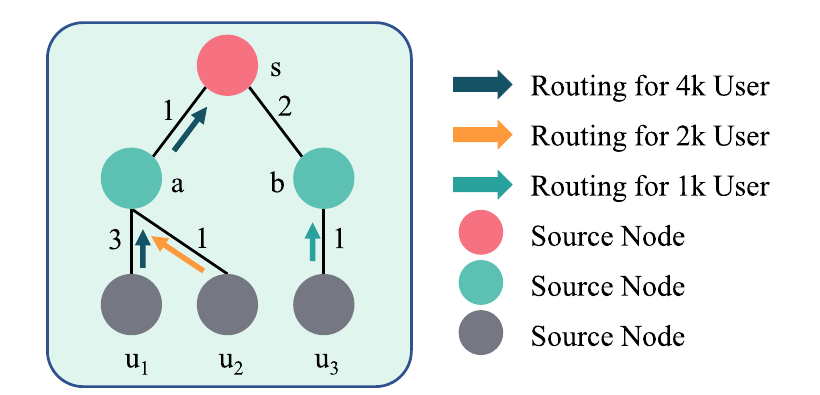
\includegraphics[width=0.5\textwidth]{fig2.png}
\caption[Routing example of the base paper (Lemma 1)]{A shared link carries the highest downstream demand (Lemma~1)~\cite{wang2026gnn}.}
\label{fig:bp_example}
\end{figure}

\begin{figure}[!htb]
\centering
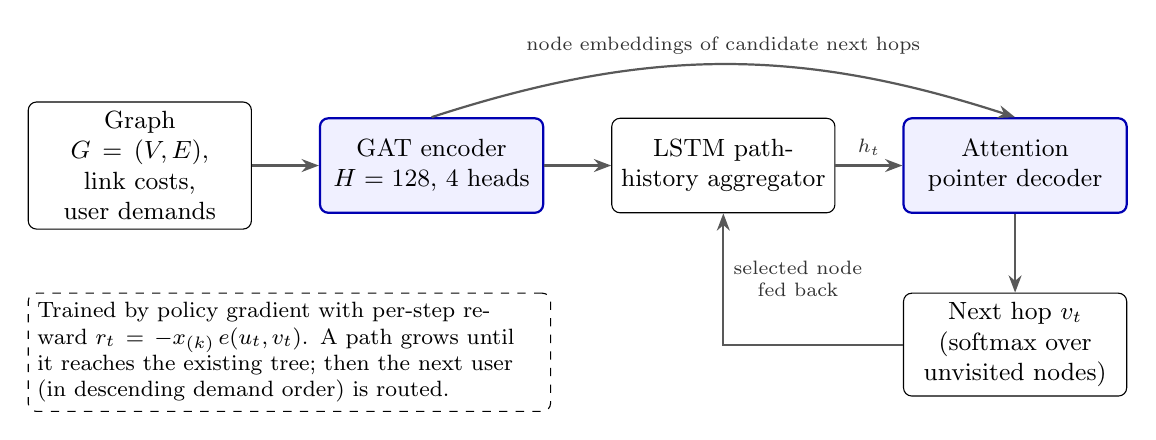
\begin{tikzpicture}[
    font=\small,
    box/.style={draw, rounded corners=3pt, align=center, minimum height=1.2cm, text width=2.6cm, fill=white},
    acc/.style={box, draw=blue!70!black, fill=blue!6, thick},
    arr/.style={-{Stealth[length=2.2mm]}, thick, gray!70!black},
    lab/.style={font=\scriptsize, text=gray!40!black, align=center}]
  \node[box] (in) {Graph $G=(V,E)$,\\link costs,\\user demands};
  \node[acc, right=0.85cm of in] (gat) {GAT encoder\\$H=128$, 4 heads};
  \node[box, right=0.85cm of gat] (lstm) {LSTM path-\\history aggregator};
  \node[acc, right=0.85cm of lstm] (dec) {Attention\\pointer decoder};
  \node[box, below=1.0cm of dec] (act) {Next hop $v_t$\\(softmax over\\unvisited nodes)};
  \node[draw, dashed, rounded corners=3pt, align=left, font=\footnotesize, text width=6.4cm, anchor=north west] (rew) at ($(in.south west)+(0,-0.8)$) {Trained by policy gradient with per-step reward $r_t=-x_{(k)}\,e(u_t,v_t)$. A path grows until it reaches the existing tree; then the next user (in descending demand order) is routed.};
  \draw[arr] (in) -- (gat);
  \draw[arr] (gat) -- (lstm);
  \draw[arr] (lstm) -- node[above, lab] {$h_t$} (dec);
  \draw[arr] (gat.north) to[bend left=18] node[above, lab] {node embeddings of candidate next hops} (dec.north);
  \draw[arr] (dec) -- (act);
  \draw[arr] (act.west) -| node[right, lab, pos=0.75] {selected node\\fed back} (lstm.south);
\end{tikzpicture}
\caption[Architecture of the base paper's graph policy network (GPN)]{Architecture of the base paper's GPN~\cite{wang2026gnn}.}
\label{fig:gpn_arch}
\end{figure}

\begin{figure}[!htb]
\centering
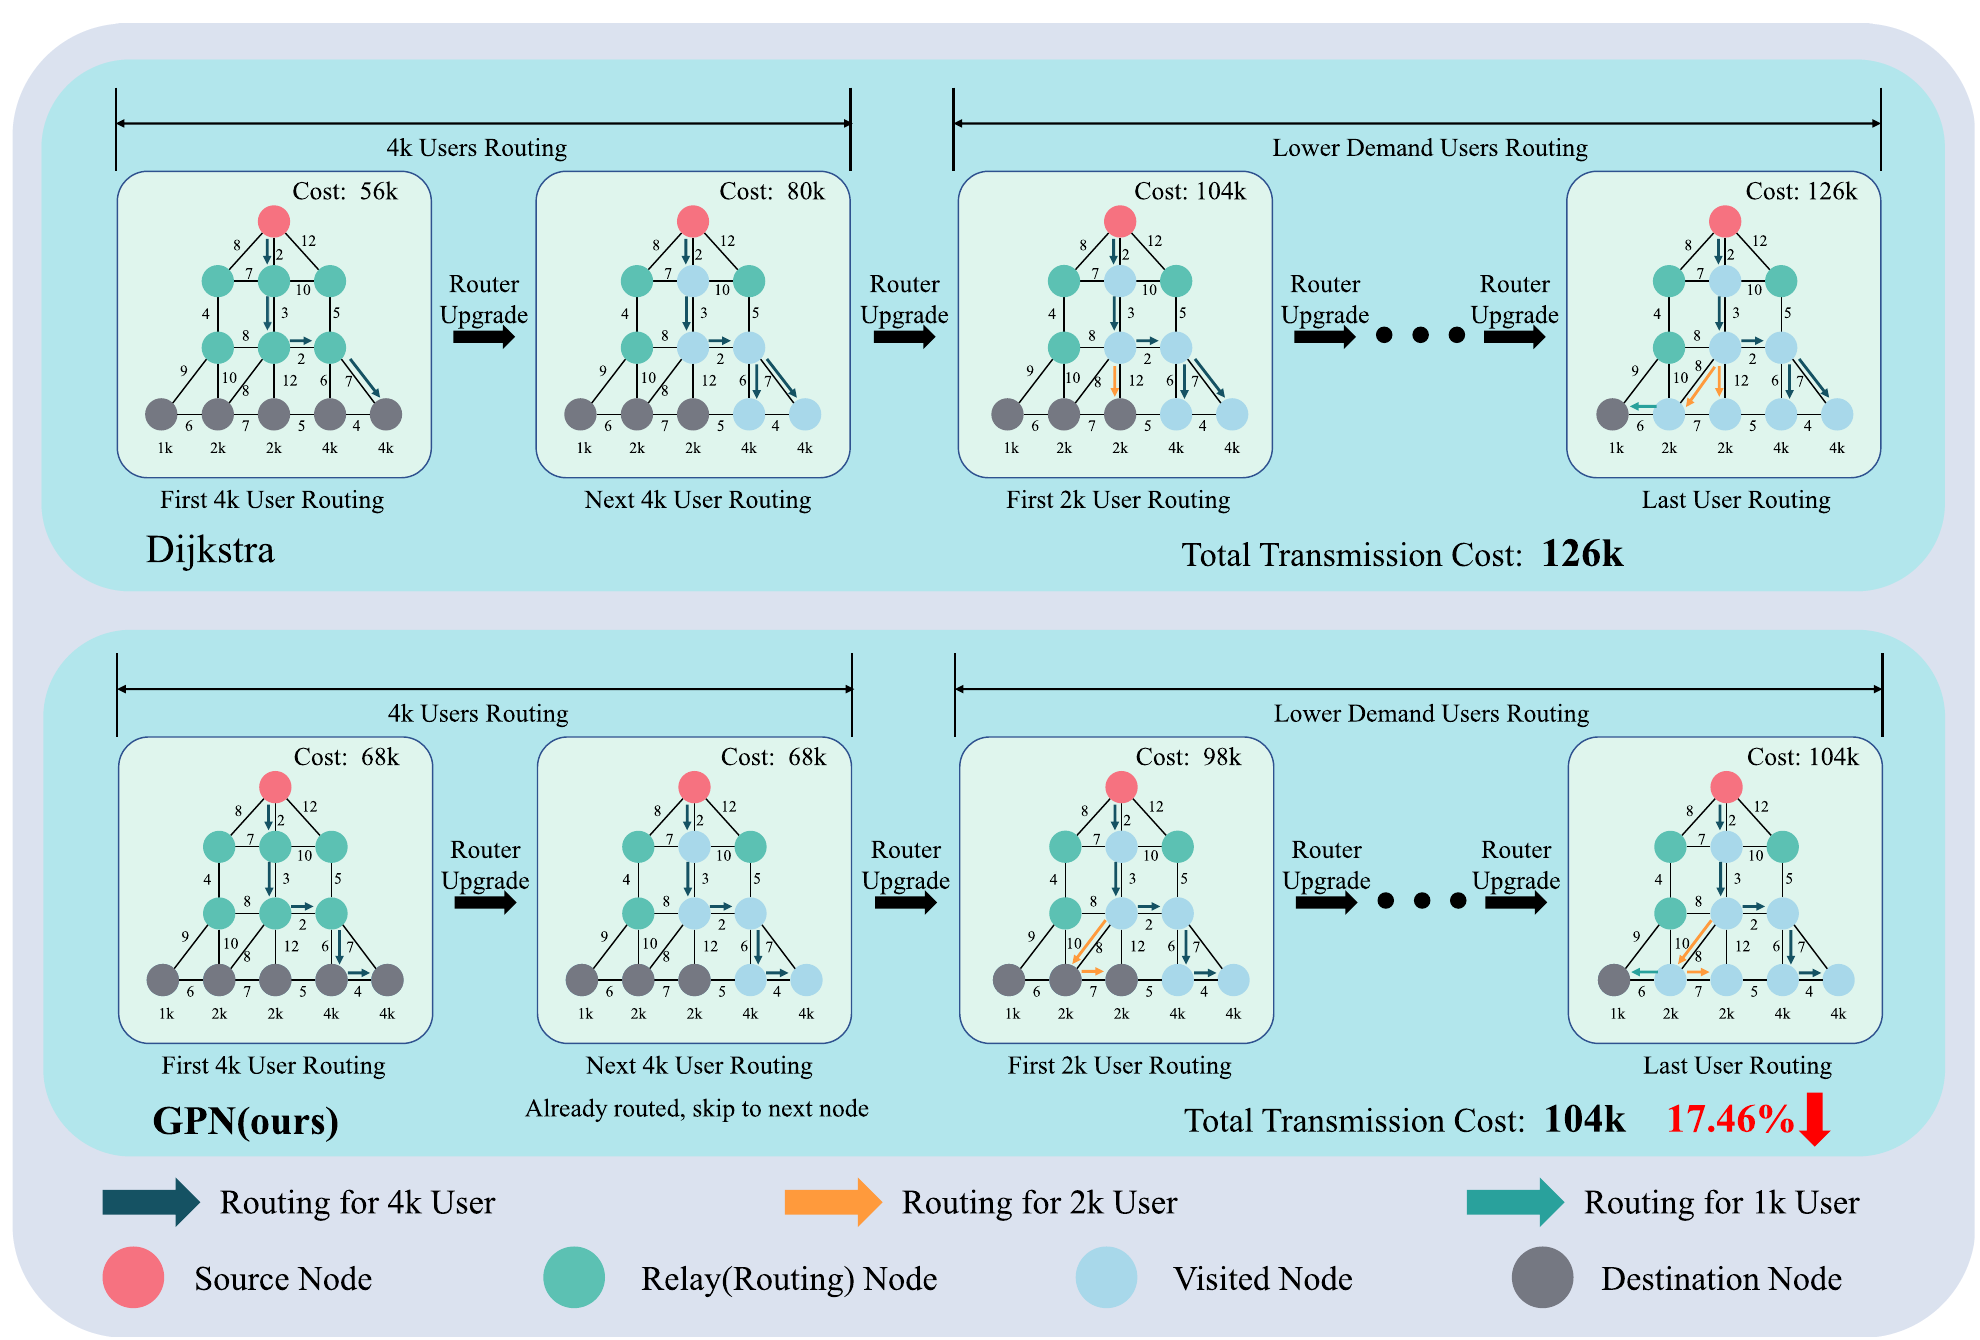
\includegraphics[width=0.92\textwidth]{fig1.png}
\caption[Sequential routing in the base paper: Dijkstra vs.\ GPN]{Routing under sequential user arrivals: Dijkstra (top) builds independent paths, while GPN (bottom) reuses branches and cuts total cost by 17.46\% in this example~\cite{wang2026gnn}.}
\label{fig:bp_sequential}
\end{figure}

\begin{figure}[!htb]
\centering
\begin{minipage}[t]{0.48\textwidth}\centering
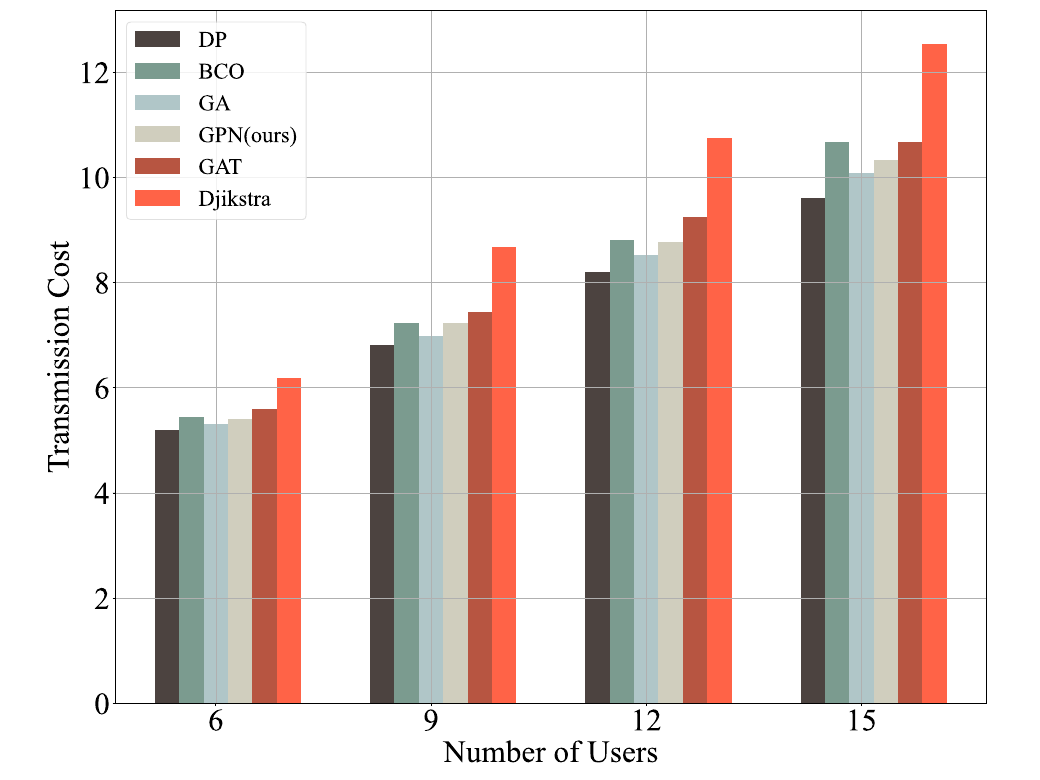
\includegraphics[width=\textwidth]{fig7.png}\\[-2pt]{\small (a) Cost vs.\ users (6--15), 50 nodes}
\end{minipage}\hfill
\begin{minipage}[t]{0.48\textwidth}\centering
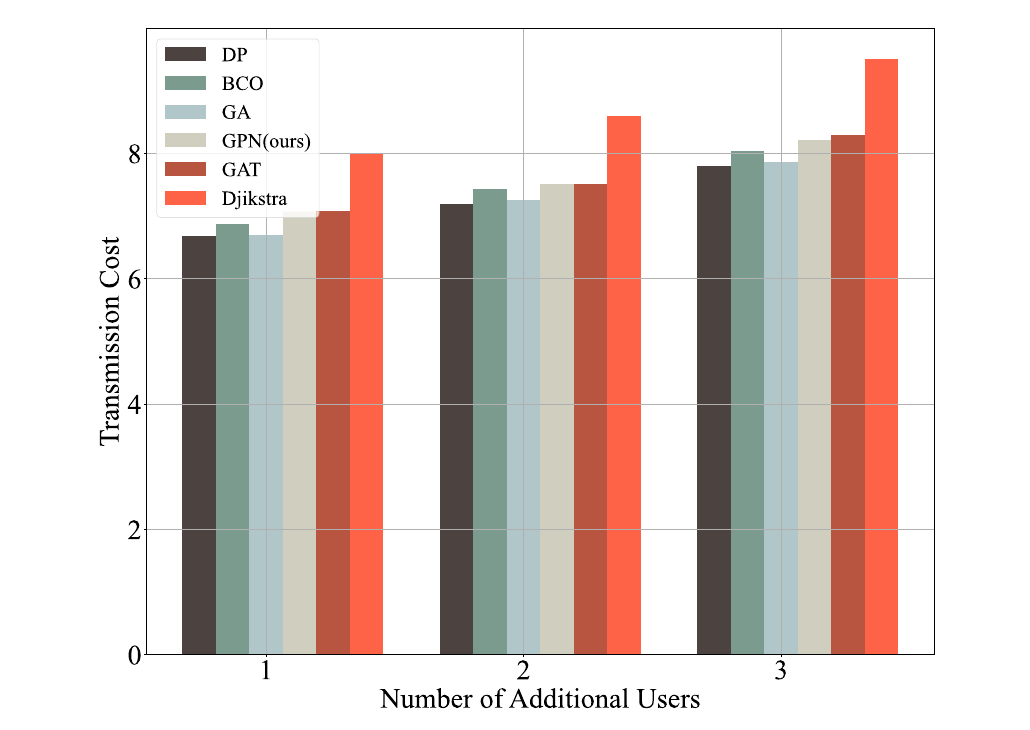
\includegraphics[width=\textwidth]{fig13.png}\\[-2pt]{\small (b) Cost after adding 1--3 users to 9}
\end{minipage}
\caption[Base paper results: cost vs.\ users and the dynamic-addition test]{Base paper results on 50-node graphs: (a) routing cost vs.\ number of users; (b) its only dynamic test~\cite{wang2026gnn}.}
\label{fig:bp_results}
\end{figure}

\noindent \textbf{Zhao \emph{et al.}}~\cite{zhao2022drlm4mr} proposed DRL-M4MR, which treats the network as four $n\times n$ matrices (tree state, residual bandwidth, delay, loss) and uses a double dueling DQN with prioritised replay to add one link per step. In Ryu/Mininet on a 14-node topology it raised bottleneck bandwidth by 19.37\% over KMB. Its limitation is that its trees used 15--30\% more links, its fixed-size matrix input ties the model to one topology, and it re-solves for a fixed destination set.

\noindent \textbf{Zhang \emph{et al.}}~\cite{zhang2026ghacmr} proposed GHAC-MR, which uses graph message passing with a PPO actor--critic and Bernoulli per-link forwarding actions, and reports lower delay and loss than KMB, GA, DRL-M4MR and a hierarchical-RL router on three topologies. Its limitation is that it also rebuilds trees for a fixed destination set without modelling leaves, quality changes or rule churn, and its own results show the hierarchical-RL router with higher bandwidth on Fat-Tree (16.74 vs.\ 14.63).

\noindent \textbf{Imase and Waxman}~\cite{imase1991dynamic} studied the dynamic Steiner tree problem and showed that a greedy online tree is $O(\log n)$-competitive as receivers join, and that a limited number of rearrangements restores a constant-factor bound when receivers also leave. This is the cost-versus-rearrangement trade-off that this thesis measures when comparing local repair with full re-planning. Its limitation is that the analysis assumes a single rate and no link capacities, and gives no learned or practical policy for when to rearrange.

\noindent \textbf{Shen \emph{et al.}}~\cite{shen2015rst} proposed the Recover-aware Steiner Tree (RST) for SDN multicast, which jointly minimises tree cost and the cost of recovering from link failures, and validated it on an SDN testbed. Its limitation is that it handles a single rate and a fixed group, and does not consider receiver churn or the cost of reconfiguring switch rules.

\noindent \textbf{Oostenbrink \emph{et al.}}~\cite{oostenbrink2017failover} pre-install backup paths as OpenFlow fast-failover groups, so switches reroute multicast traffic locally without the controller and recover in under 10\,ms. Its limitation is the extra switch memory for backup state, and the trees it protects are classical single-rate trees rather than learned multi-rate ones.

\noindent \textbf{Reitblatt \emph{et al.}}~\cite{reitblatt2012update} introduced two-phase, versioned rule updates that guarantee each packet is processed by either the old or the new configuration, never a mix. Its limitation, for this thesis, is that it makes a change safe but not cheap: it does not decide which tree to install or how many rules to change.

\noindent Table~\ref{tab:comparison} compares these works with this thesis.

\begin{table}[!htb]
\caption{Comparison of the related works}
\label{tab:comparison}
\begin{center}
\footnotesize
\renewcommand{\arraystretch}{1.1}
\begin{tabular}{|L{2.3cm}|L{2.4cm}|C{1.2cm}|L{1.8cm}|L{1.8cm}|L{1.9cm}|L{2.1cm}|}
\hline
\textbf{Work} & \textbf{Tree builder} & \textbf{Multi-rate} & \textbf{Leave / quality change} & \textbf{Link failure} & \textbf{Rule-change cost} & \textbf{Validation} \\
\hline\hline
MPH / KMB~\cite{takahashi1980mph,kou1981kmb} & Heuristic, $2(1-1/l)$ bound & No & Full re-plan & Full re-plan & Not measured & Analysis \\ \hline
Online Steiner~\cite{imase1991dynamic} & Greedy + rearrangement & No & Yes (theory) & No & Edge changes bounded & Analysis \\ \hline
DRL-M4MR~\cite{zhao2022drlm4mr} & Double dueling DQN & No & No & No & No & Ryu + Mininet, 14 nodes \\ \hline
GHAC-MR~\cite{zhang2026ghacmr} & GNN + PPO & No & No & No & No & Ryu + Mininet, 3 topologies \\ \hline
RST~\cite{shen2015rst} & Approximation & No & No & Yes (recovery cost) & No & SDN testbed \\ \hline
Fast-failover~\cite{oostenbrink2017failover} & Precomputed backups & No & Join/leave groups & Yes, $<$10\,ms & Switch memory & Emulation \\ \hline
Base paper~\cite{wang2026gnn} & GAT + LSTM pointer & Yes & Adds only & No & No & Simulation, $\le$50 nodes \\ \hline
\textbf{This thesis} & Base GPN + repair operators + MPH net & Yes & Yes & Yes, fast-failover & Yes ($\mu\times$ changes) & Simulation, Mininet/Ryu, 5G SA lab \\
\hline
\end{tabular}
\end{center}
\end{table}

\section{Research Gaps}\label{sec:lr_gap}
\noindent Learned multi-rate multicast has been shown to build good trees, but not to keep them cheap, stable and protected while the audience and the network change, and not at real receivers. The specific gaps found in the literature review are:
\begin{itemize}
    \item \textbf{Viewers leaving or lowering quality} are not modelled; only 1--3 additions are tested, so unused branches keep consuming bandwidth (addressed by the cost model and the repair operators).
    \item \textbf{Late high-quality joins} are under-priced, because the reward charges only newly added links and ignores upstream upgrades (addressed by the cost model).
    \item \textbf{Link failures and mobility} are never tested; the only recovery is a full re-plan (addressed by the repair operators and fast-failover protection).
    \item \textbf{Link capacity} is not constrained, so congestion is invisible to the model (addressed by the capacity-constrained formulation).
    \item \textbf{Reconfiguration cost} is ignored: there is no control plane, and a re-plan re-routes every user, so rule churn and video disruption are unmeasured (addressed by the rule-change penalty and two-phase updates).
    \item \textbf{No quality guarantee}: GPN is 6--7\% above optimum and was never compared with Steiner heuristics; our replication finds layered MPH at least as cheap on about 80\% of instances (addressed by the MPH safety net of the learned policy).
    \item \textbf{Evaluation} uses random graphs of at most 50 nodes, and ``delay'' means computation time, so there is no evidence at real switches or users (addressed by the three-tier evaluation).
\end{itemize}

\section{Problem Formulation}\label{sec:lr_rq}
\noindent The problem addressed by this thesis is:
\begin{itemize}
    \item Given an SDN transport network with link capacities, a video source with cumulative quality layers, and a stream of events (join, leave, quality change, link or switch failure), maintain a multi-rate multicast tree that minimises tree cost plus a penalty on rule changes, while keeping video disruption at receivers low.
\end{itemize}
\noindent The work answers three research questions:
\begin{itemize}
    \item Under realistic join, leave, quality-change and failure patterns, how many rule changes and how much recomputation do local repair operators save versus full re-planning, and at what tree-cost penalty?
    \item Can the base paper's GNN, extended to choose keep / local repair / full re-plan and paired with a certified MPH fallback, beat fixed-threshold policies on combined cost and churn?
    \item Do pre-installed backup paths measurably reduce video disruption at real 5G UEs, and how much extra switch state do they cost?
\end{itemize}


\chapter{Proposed Methodology}\label{chap:methodology}
\vspace{-1cm}
\noindent \rule{6.6in}{0.01in}
\emph{This chapter describes the proposed event-driven tree-maintenance method and its control loop. Section~\ref{sec:m_formulation} formulates the problem, with the tree cost model, the rule-change penalty and correct upgrade cost accounting. Section~\ref{sec:m_operators} defines the local repair operators. Section~\ref{sec:m_policy} presents the learned keep/repair/re-plan policy and the capacity-aware layered MPH safety net that bounds its cost. Section~\ref{sec:m_protection} covers fast-failover backup branches and two-phase rule updates, and Section~\ref{sec:m_evaluation} describes the three-tier evaluation in simulation, emulation and the 5G lab.}
\noindent The method keeps the base paper's GNN as the tree builder and wraps it in an event-driven maintenance loop (Figure~\ref{fig:control_loop}). Each event is handled by keeping the tree, repairing it locally or re-planning it; the installed tree never costs more than $(1+\varepsilon)$ times a capacity-aware layered MPH tree; and changes reach the switches through protected, two-phase updates.

\begin{figure}[!htb]
\centering
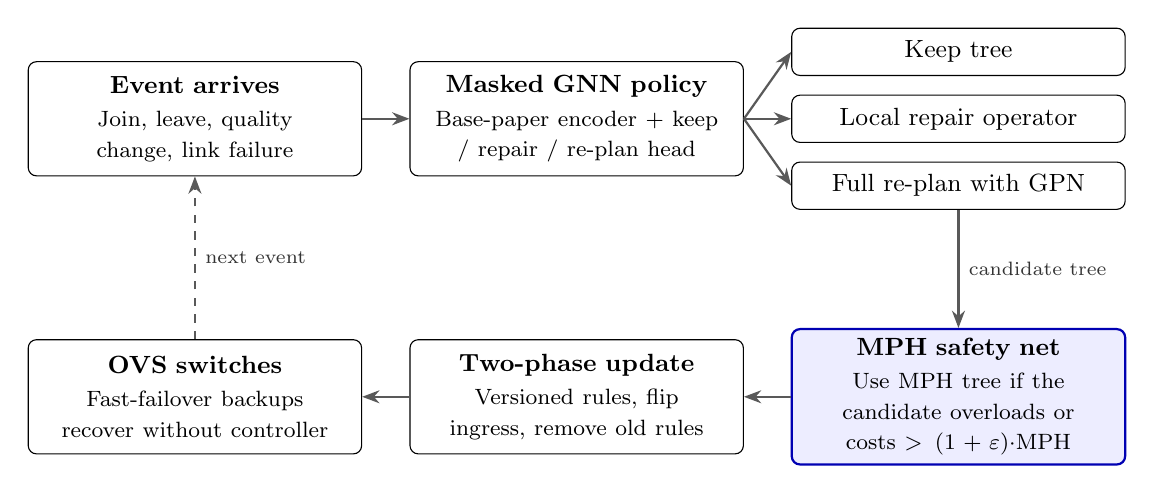
\begin{tikzpicture}[
    font=\small,
    box/.style={draw, rounded corners=3pt, align=center, minimum height=1.45cm, text width=4.0cm, fill=white},
    opt/.style={draw, rounded corners=3pt, align=center, minimum height=0.6cm, text width=4.0cm, fill=white},
    acc/.style={box, draw=blue!70!black, fill=blue!7, thick},
    arr/.style={-{Stealth[length=2.2mm]}, thick, gray!70!black},
    lab/.style={font=\scriptsize, text=gray!40!black}]
  \node[box] (ev) {\textbf{Event arrives}\\[1pt]{\footnotesize Join, leave, quality change, link failure}};
  \node[box, right=0.6cm of ev] (pol) {\textbf{Masked GNN policy}\\[1pt]{\footnotesize Base-paper encoder + keep / repair / re-plan head}};
  \node[opt, right=0.6cm of pol, yshift=0.85cm] (keep) {Keep tree};
  \node[opt, right=0.6cm of pol] (rep) {Local repair operator};
  \node[opt, right=0.6cm of pol, yshift=-0.85cm] (re) {Full re-plan with GPN};
  \node[acc, below=1.5cm of re] (mph) {\textbf{MPH safety net}\\[1pt]{\footnotesize Use MPH tree if the candidate overloads or costs $>(1+\varepsilon)\cdot$MPH}};
  \node[box] (upd) at (pol |- mph) {\textbf{Two-phase update}\\[1pt]{\footnotesize Versioned rules, flip ingress, remove old rules}};
  \node[box] (ovs) at (ev |- mph) {\textbf{OVS switches}\\[1pt]{\footnotesize Fast-failover backups recover without controller}};
  \draw[arr] (ev) -- (pol);
  \draw[arr] (pol.east) -- (keep.west);
  \draw[arr] (pol.east) -- (rep.west);
  \draw[arr] (pol.east) -- (re.west);
  \draw[arr] (re) -- node[right, lab] {candidate tree} (mph);
  \draw[arr] (mph) -- (upd);
  \draw[arr] (upd) -- (ovs);
  \draw[arr, dashed] (ovs) -- node[right, lab] {next event} (ev);
\end{tikzpicture}
\caption[Event-driven tree maintenance loop]{Event-driven tree maintenance loop: the learned policy chooses how much to change, the MPH check bounds the cost, and switches handle failures locally until the controller's repair arrives.}
\label{fig:control_loop}
\end{figure}

\section{Problem Formulation}\label{sec:m_formulation}
\noindent The network is a graph $G=(V,E)$ with unit cost $e_{ij}$ and capacity $c_{ij}$ per link. A session has a source $s$ and receivers $k$ with cumulative quality demand $x_k \in \{0.25, 0.5, 1.0\}$, as in~\cite{wang2026gnn}. By Lemma~1 of~\cite{wang2026gnn}, a tree link carries the highest demand below it, so the cost of a tree $T$ is
\begin{equation}
C(T) = \sum_{(i,j) \in T} e_{ij}\, f_{ij}, \qquad f_{ij} = \max_{k \in \mathcal{D}_T(j)} x_k, \qquad f_{ij} \le c_{ij},
\label{eq:tree_cost}
\end{equation}
where $\mathcal{D}_T(j)$ is the set of receivers downstream of $j$. After each event $t$ the controller chooses a new tree $T_t$ that minimises tree cost plus a penalty on rule changes:
\begin{equation}
\min_{T_t}\; C(T_t) + \mu \,\bigl| R(T_t) \,\triangle\, R(T_{t-1}) \bigr| ,
\label{eq:objective}
\end{equation}
where $R(T)$ is the set of OpenFlow rules that realise $T$ and $\mu$ prices one rule change; sweeping $\mu$ traces the cost-versus-churn curve used to compare local repair with full re-planning. The base paper's reward charges only new links. When a receiver with demand $x_k$ grafts onto the tree at node $a$, the true marginal cost also includes raising every upstream link on the path $P(s,a)$:
\begin{equation}
\Delta C = \sum_{(i,j) \in \text{new}} e_{ij}\, x_k \;+\; \sum_{(i,j) \in P(s,a)} e_{ij}\,\bigl(\max(f_{ij}, x_k) - f_{ij}\bigr).
\label{eq:delta_cost}
\end{equation}
A leave or downgrade runs the same rule in reverse: $f$ is recomputed upward from the leaf, and links with no receivers below are pruned.

\section{Repair Operators}\label{sec:m_operators}
\noindent Table~\ref{tab:operators} lists the operators, which run inside a Ryu controller module that tracks the current tree, link loads and installed rules.

\begin{table}[!htb]
\caption{Repair operators}
\label{tab:operators}
\begin{center}
\footnotesize
\renewcommand{\arraystretch}{1.1}
\begin{tabular}{|L{2.4cm}|L{2.4cm}|L{6.2cm}|L{3.2cm}|}
\hline
\textbf{Operator} & \textbf{Triggered by} & \textbf{Action} & \textbf{Rules touched} \\
\hline\hline
Graft & Join & Attach the receiver at the tree node with least marginal cost $\Delta C$ (Eq.~\ref{eq:delta_cost}) & New branch + upstream upgrades \\ \hline
Prune-up & Leave & Remove the leaf branch up to the first node that still serves a receiver & Removed branch only \\ \hline
Layer upgrade / downgrade & Quality change & Re-propagate $f$ along the path to the source & Group memberships on that path \\ \hline
Re-attach & Link or switch failure & Reconnect each orphaned subtree by its cheapest path & Orphaned subtrees' new paths \\ \hline
Full re-plan & Policy choice or cost drift & Rebuild with GPN, then apply the MPH check & All changed rules \\
\hline
\end{tabular}
\end{center}
\end{table}

\section{Learned Decision Policy and MPH Safety Net}\label{sec:m_policy}
\noindent The base GPN encoder (Figure~\ref{fig:gpn_arch}) is reused with extra node features (in-tree flag, current $f$ on the parent link, residual capacity, event type), and a small masked head chooses keep, local repair or full re-plan; for example, keep is masked after a failure that disconnects a receiver. The head is trained by policy gradient on simulated event traces with reward equal to the negative of Eq.~\eqref{eq:objective}. Baselines for the learned policy are fixed-threshold rules (always repair; re-plan when cost drifts more than $\tau\%$ above MPH; re-plan every $N$ events), all re-planning with MPH, and the main baseline for the repair operators is a full MPH re-plan per event. Whatever the policy chooses, the resulting tree passes the MPH check of Algorithm~\ref{alg:mph} before it is installed.

\begin{algorithm}[!htb]
\caption{Capacity-aware layered MPH and install rule (one session)}
\label{alg:mph}
\begin{algorithmic}[1]
\For{layer $x \in \{1.0,\ 0.5,\ 0.25\}$} \Comment{highest rate first}
  \State $G_x \gets$ links with residual $+$ own\_load $\ge x$ \Comment{own\_load: this session's current use}
  \While{some layer-$x$ receiver $r$ is unconnected}
    \State attach the $r$ whose cheapest path to the current tree in $G_x$ is cheapest
    \State \hspace{1em}(tree links cost 0, new links cost $e_{ij}$)
  \EndWhile
  \If{$r$ cannot reach the tree in $G_x$}
    \State retry $r$ at the next lower layer; drop it only if none works
  \EndIf
\EndFor
\If{candidate does not fit the residual capacities}
  \State install the MPH tree
\ElsIf{$C(\text{candidate}) > (1+\varepsilon)\, C(\text{MPH tree})$}
  \State install the MPH tree
\Else
  \State install the candidate
\EndIf
\end{algorithmic}
\end{algorithm}

\noindent Adding layers from the highest rate down means a later, lower layer never raises the load on a link already in the tree, so the per-layer pruning is exact: for one session, MPH finds a tree that fits whenever one exists, and a receiver it must downgrade cannot be served at its rate by any tree. The tolerance $\varepsilon$ stops every MPH win from becoming a full re-plan, the churn that $\mu$ penalises. With no binding capacity, the installed tree costs at most $(1+\varepsilon)$ times the layered MPH tree, which is within $\frac{\ell+1}{2}\rho$ of optimal~\cite{ahmed2019mlst}, about $4\times$ for three layers. That proof prices a link by the number of layers crossing it, so the bound must be re-derived for the unevenly spaced rates 0.25/0.5/1.0, or layered MPH replaced by the $e\cdot\rho$ algorithm of~\cite{charikar2004qos}. Whether the bound holds when capacity binds is not yet proven, and several sessions sharing links are not covered. The net's value lies in capping the drift of repeated local repairs, which as greedy online updates can drift to $O(\log n)$ times optimal~\cite{imase1991dynamic}.

\section{Proactive Protection and Safe Updates}\label{sec:m_protection}
\noindent For each tree link, a backup path to the downstream subtree is installed as an OpenFlow~1.3 fast-failover group~\cite{oostenbrink2017failover}, so the switch fails over without the controller; backups share tree links where possible to limit extra state. New rules are installed under a new version tag, the ingress is flipped to that tag, and old rules are removed after a timeout~\cite{reitblatt2012update}, so each receiver sees either the old or the new tree. Recovery time, packets lost during failover and extra flow and group entries per switch are measured.

\section{Three-Tier Evaluation}\label{sec:m_evaluation}
\noindent The method is evaluated in three tiers (Table~\ref{tab:tiers}). Because the lab's Release 15/16 system has no 5G MBS~\cite{3gpp23247}, the tree ends at the MEC replicator and the last hop is one unicast PDU session per UE (Figure~\ref{fig:testbed}); extra edge sites are emulated with Open5GS and UERANSIM, and the lab's core and RAN settings are never changed.

\begin{table}[!htb]
\caption{Three-tier evaluation plan}
\label{tab:tiers}
\begin{center}
\footnotesize
\renewcommand{\arraystretch}{1.1}
\begin{tabular}{|L{1.9cm}|L{6.0cm}|L{2.5cm}|L{3.8cm}|}
\hline
\textbf{Tier} & \textbf{Setup} & \textbf{Scale} & \textbf{Measures} \\
\hline\hline
1 Simulation & Event-driven Python/NetworkX simulator; Topology Zoo, Rocketfuel and the base paper's random graphs & 50--500 nodes, thousands of events & Cost vs.\ churn, policy training, scalability \\ \hline
2 Emulation & Mininet + Open vSwitch + the Ryu module; UDP flows at layer rates & Tens of switches & Rule churn, recovery time, switch state \\ \hline
3 5G lab & Emulated transport attached through the lab switch (dedicated VLAN) to the 5G SA core; MEC hosts the edge replicator & Lab CPEs and XR headsets & Stalls, startup delay, frame loss at real UEs \\
\hline
\end{tabular}
\end{center}
\end{table}

\begin{figure}[!htb]
\centering
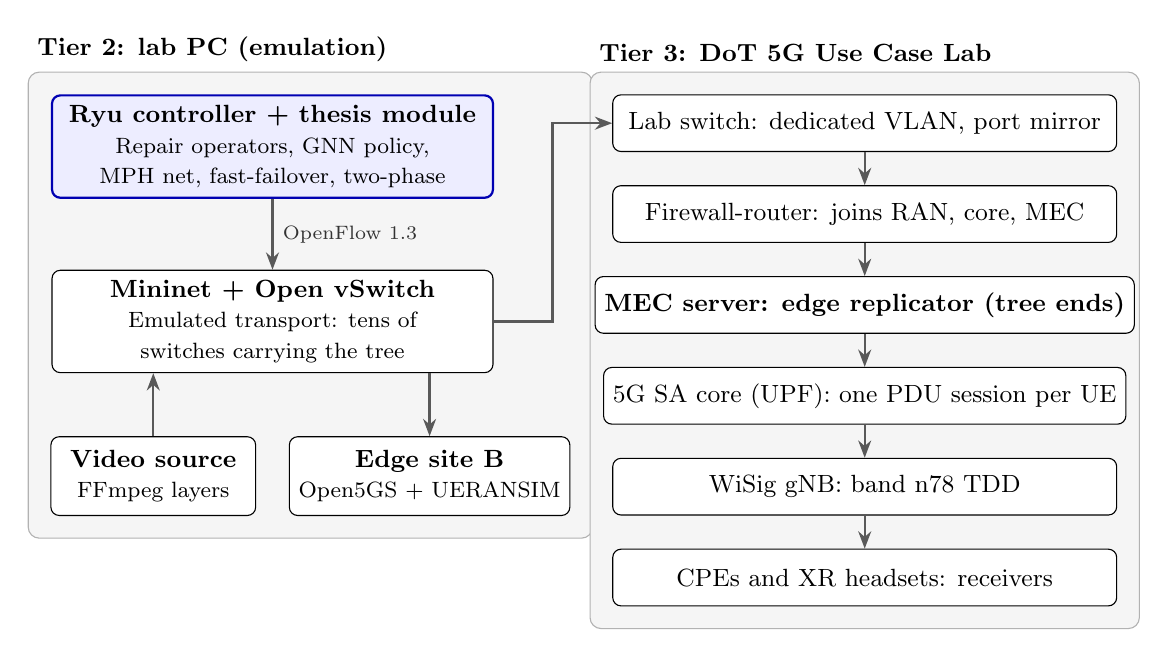
\begin{tikzpicture}[
    font=\small,
    box/.style={draw, rounded corners=3pt, align=center, fill=white},
    acc/.style={box, draw=blue!70!black, fill=blue!7, thick},
    chain/.style={box, minimum width=6.4cm, minimum height=0.72cm},
    arr/.style={-{Stealth[length=2.2mm]}, thick, gray!70!black},
    lab/.style={font=\scriptsize, text=gray!40!black}]
  % Tier 2
  \node[acc, minimum width=5.6cm, minimum height=1.3cm] (ryu) at (0,0) {\textbf{Ryu controller + thesis module}\\{\footnotesize Repair operators, GNN policy,}\\{\footnotesize MPH net, fast-failover, two-phase}};
  \node[box, minimum width=5.6cm, minimum height=1.3cm, below=0.9cm of ryu] (ovs) {\textbf{Mininet + Open vSwitch}\\{\footnotesize Emulated transport: tens of}\\{\footnotesize switches carrying the tree}};
  \node[box, minimum width=2.6cm, minimum height=1.0cm, below left=0.8cm and -2.6cm of ovs] (src) {\textbf{Video source}\\{\footnotesize FFmpeg layers}};
  \node[box, minimum width=2.6cm, minimum height=1.0cm, below right=0.8cm and -2.6cm of ovs] (edgeb) {\textbf{Edge site B}\\{\footnotesize Open5GS + UERANSIM}};
  \draw[arr] (ryu) -- node[right, lab] {OpenFlow 1.3} (ovs);
  \draw[arr] (src) -- (src |- ovs.south);
  \draw[arr] (edgeb |- ovs.south) -- (edgeb);
  \begin{scope}[on background layer]
    \node[draw=gray!60, fill=gray!8, rounded corners=4pt, inner sep=8pt, fit=(ryu)(ovs)(src)(edgeb), label={[font=\small\bfseries, anchor=south west]north west:Tier 2: lab PC (emulation)}] (t2) {};
  \end{scope}
  % Tier 3
  \node[chain, right=1.5cm of ryu.north east, anchor=north west] (c1) {Lab switch: dedicated VLAN, port mirror};
  \node[chain, below=0.42cm of c1] (c2) {Firewall-router: joins RAN, core, MEC};
  \node[chain, below=0.42cm of c2, font=\small\bfseries] (c3) {MEC server: edge replicator (tree ends)};
  \node[chain, below=0.42cm of c3] (c4) {5G SA core (UPF): one PDU session per UE};
  \node[chain, below=0.42cm of c4] (c5) {WiSig gNB: band n78 TDD};
  \node[chain, below=0.42cm of c5] (c6) {CPEs and XR headsets: receivers};
  \foreach \a/\b in {c1/c2,c2/c3,c3/c4,c4/c5,c5/c6} \draw[arr] (\a) -- (\b);
  \begin{scope}[on background layer]
    \node[draw=gray!60, fill=gray!8, rounded corners=4pt, inner sep=8pt, fit=(c1)(c6), label={[font=\small\bfseries, anchor=south west]north west:Tier 3: DoT 5G Use Case Lab}] (t3) {};
  \end{scope}
  \draw[arr] (ovs.east) -- ++(0.75,0) |- (c1.west);
\end{tikzpicture}
\caption[Tier 2--3 testbed architecture]{Tier 2--3 testbed: the multicast tree runs in Open vSwitch up to the MEC replicator; the 5G system carries only the unicast last hop. The thesis builds only the highlighted module.}
\label{fig:testbed}
\end{figure}

\noindent Workloads use Poisson viewer arrivals, exponential viewing times and Zipf audience sizes, with demand split one-third high, medium and low as in~\cite{wang2026gnn}, plus random and correlated link and switch failures. Metrics are tree cost (and gap to an exact ILP up to about 50 nodes), rule changes per event, decision time, recovery time, extra switch entries and, at Tier~3, stall count, stall duration and startup delay. All tools are open source: PyTorch Geometric with the base paper's code, OR-Tools/SCIP, Ryu, Mininet, Open vSwitch, Open5GS, UERANSIM and FFmpeg.


\chapter{Results and Discussion}\label{chap:results}
\vspace{-1cm}
\noindent \rule{6.6in}{0.01in}
\emph{This chapter reports the experiments carried out so far. Section~\ref{sec:r_setup} describes the replication setup: the public code, the fixes applied, the datasets and the hardware. Section~\ref{sec:r_reproduction} presents the training curves and the reproduced cost ratios against the paper's figures. Section~\ref{sec:r_baselines} compares GPN with classical Steiner heuristics in cost and run time. Section~\ref{sec:r_discussion} discusses what these findings mean for the thesis, Section~\ref{sec:c_conclusions} draws the conclusions of the mid-term work, and Section~\ref{sec:c_future} sets out the future scope.}
\section{Replication Setup}\label{sec:r_setup}
\noindent The base paper was replicated from its public code (Figure~\ref{fig:repro_pipeline}). The paper's model, generator and reward were left untouched; every change sits in device handling, training speed or evaluation (Table~\ref{tab:repro_setup}).

\begin{figure}[!htb]
\centering
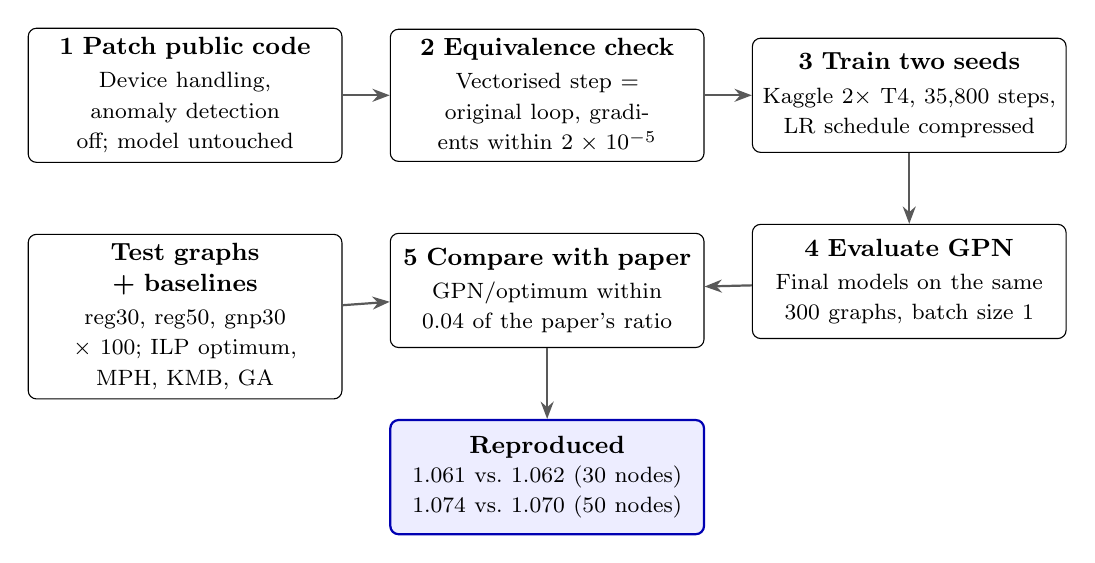
\begin{tikzpicture}[
    font=\small,
    box/.style={draw, rounded corners=3pt, align=center, minimum height=1.45cm, text width=3.75cm, fill=white},
    acc/.style={box, draw=blue!70!black, fill=blue!7, thick},
    arr/.style={-{Stealth[length=2.2mm]}, thick, gray!70!black}]
  \node[box] (p1) {\textbf{1 Patch public code}\\[1pt]{\footnotesize Device handling, anomaly detection off; model untouched}};
  \node[box, right=0.6cm of p1] (p2) {\textbf{2 Equivalence check}\\[1pt]{\footnotesize Vectorised step = original loop, gradients within $2\times10^{-5}$}};
  \node[box, right=0.6cm of p2] (p3) {\textbf{3 Train two seeds}\\[1pt]{\footnotesize Kaggle $2\times$ T4, 35,800 steps, LR schedule compressed}};
  \node[box, below=0.9cm of p3] (p4) {\textbf{4 Evaluate GPN}\\[1pt]{\footnotesize Final models on the same 300 graphs, batch size 1}};
  \node[box, below=0.9cm of p2] (p5) {\textbf{5 Compare with paper}\\[1pt]{\footnotesize GPN/optimum within 0.04 of the paper's ratio}};
  \node[box, below=0.9cm of p1] (tb) {\textbf{Test graphs + baselines}\\[1pt]{\footnotesize reg30, reg50, gnp30 $\times$ 100; ILP optimum, MPH, KMB, GA}};
  \node[acc, below=0.9cm of p5] (v) {\textbf{Reproduced}\\[1pt]{\footnotesize 1.061 vs.\ 1.062 (30 nodes)\\1.074 vs.\ 1.070 (50 nodes)}};
  \draw[arr] (p1) -- (p2); \draw[arr] (p2) -- (p3); \draw[arr] (p3) -- (p4);
  \draw[arr] (p4) -- (p5); \draw[arr] (tb) -- (p5); \draw[arr] (p5) -- (v);
\end{tikzpicture}
\caption[Replication pipeline]{Replication pipeline: the public code reproduces the paper once patched and checked.}
\label{fig:repro_pipeline}
\end{figure}

\begin{table}[!htb]
\caption{Replication setup compared with the base paper}
\label{tab:repro_setup}
\begin{center}
\footnotesize
\renewcommand{\arraystretch}{1.1}
\begin{tabular}{|L{2.3cm}|L{5.0cm}|L{7.0cm}|}
\hline
\textbf{Item} & \textbf{Paper~\cite{wang2026gnn}} & \textbf{This replication} \\
\hline\hline
Code & Public repo (UNIC-Lab/GNN-Routing) & Same repo, commit \texttt{ce64a61}; device handling patched, anomaly detection off \\ \hline
Training & 29 nodes + hub, 9 users, ER $p=0.10$; GAT ($H=128$, 4 heads) + LSTM + pointer; Adam $5\times10^{-4}$; 50,000 steps, batch 16 & Same graphs and model; 35,800 steps (72\%) with the LR schedule compressed so the final LR factor matches (0.0169); two seeds \\ \hline
Hardware & Xeon 4214R + RTX 3090 & Kaggle, $2\times$ T4, 7.6\,h per seed; vectorised training step checked equal to the original (gradients within $2\times10^{-5}$), 11--20$\times$ faster \\ \hline
Test graphs & 30 and 50 nodes, degree 4, 12 users, 100 graphs & 4-regular 30 and 50 nodes (reg30, reg50) and the repo's ER $p=0.1$ at 30 nodes (gnp30); 12 users; 100 graphs each \\ \hline
Optimum & Dynamic programming & Layered directed Steiner ILP (HiGHS); all 300 instances proven optimal \\ \hline
Baselines & Dijkstra, GA, BCO, DP, GAT & Dijkstra, GA, layered MPH, KMB (own implementations) \\ \hline
Pass criterion & -- & GPN/optimum within 0.04 of the paper's ratio, fixed in advance \\
\hline
\end{tabular}
\end{center}
\end{table}

\noindent The public code needed several fixes: it has no baseline implementations; it hard-codes \texttt{.cuda(2)} and absolute paths; anomaly detection is on globally, slowing training several times; its validation stop check uses the training batch's features; the paper says ``degree 4'' while the test script uses ER $p=0.1$ (both were evaluated, and 4-regular graphs match the paper's optimum, 6.787 vs.\ 6.781); and the original training loop was too slow for the free GPU quota, so a vectorised step and a compressed LR schedule were used.

\section{Training and Reproduction}\label{sec:r_reproduction}
\noindent Validation cost levelled off by about step 10,000 in both seeds (Figure~\ref{fig:val_curve}), and no step was skipped for a non-finite loss. The final models are reported, since the best checkpoints were selected on validation data.

\begin{figure}[!htb]
\centering
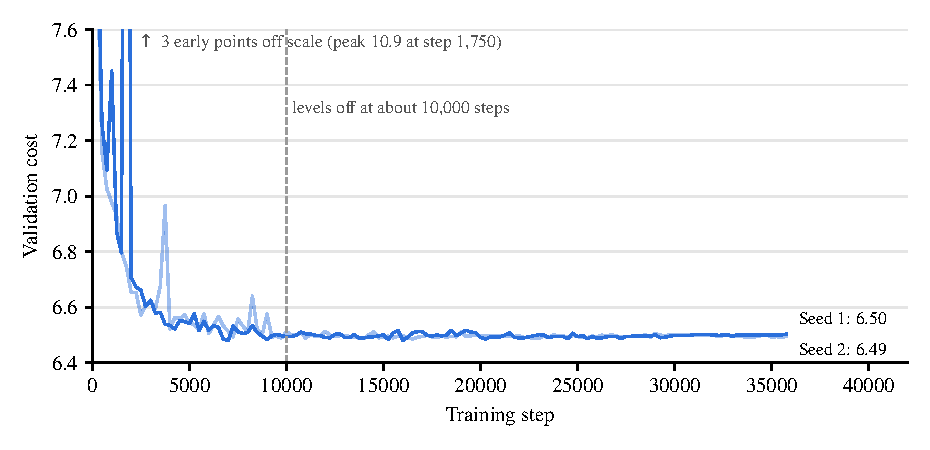
\includegraphics[width=0.75\textwidth]{validation_curve.pdf}
\caption[Validation cost during training (two seeds)]{Validation cost on 64 fixed graphs, every 250 steps, levels off by about step 10,000 in both seeds (run length 35,800 steps; paper: 50,000).}
\label{fig:val_curve}
\end{figure}

\begin{table}[!htb]
\caption{Reproduction of the base paper's headline numbers}
\label{tab:repro_main}
\begin{center}
\footnotesize
\setlength{\tabcolsep}{4pt}
\renewcommand{\arraystretch}{1.1}
\begin{tabular}{|c|C{2.0cm}|C{1.6cm}|C{1.2cm}|C{1.2cm}|C{1.7cm}|C{1.7cm}|L{2.4cm}|}
\hline
\textbf{Setting} & \textbf{Optimum (ours, 95\% CI)} & \textbf{Optimum (paper)} & \textbf{GPN (ours)} & \textbf{GPN (paper)} & \textbf{GPN / optimum (ours)} & \textbf{GPN / optimum (paper)} & \textbf{Verdict} \\
\hline\hline
reg30 & 6.806 $\pm$ 0.117 & 6.781 & 7.213 & 7.200 & 1.061 & 1.062 & Reproduced \\ \hline
reg50 & 8.333 $\pm$ 0.138 & 8.207 & 8.949 & 8.781 & 1.074 & 1.070 & Reproduced \\ \hline
gnp30 & 7.049 & -- & 7.448 & -- & 1.058 & -- & Repo's test generator \\
\hline
\end{tabular}
\end{center}
\end{table}

\noindent The paper's result is reproduced (Table~\ref{tab:repro_main}): GPN costs $1.061\times$ optimal on 30-node graphs (paper: 1.062) and $1.074\times$ on 50-node graphs (paper: 1.070), well inside the 0.04 criterion, and our exact optima agree with the paper's within their confidence intervals. Costs are means over 100 graphs, averaged over two seeds; the per-seed ratios (1.0596--1.0760) differ by at most 0.004, so the result does not hinge on one seed.

\section{Comparison with Classical Baselines}\label{sec:r_baselines}
\noindent The paper does not compare GPN against Steiner heuristics. Layered MPH is the cheapest heuristic in every setting, and GPN is the most expensive method apart from Dijkstra (Table~\ref{tab:repro_baselines}). On 50-node graphs MPH is closest to the optimum and about $45\times$ faster than GPN (Figure~\ref{fig:cost_time}); at 30 nodes it is about $65\times$ faster.

\begin{table}[!htb]
\caption{Mean tree cost over 100 graphs per setting}
\label{tab:repro_baselines}
\begin{center}
\footnotesize
\renewcommand{\arraystretch}{1.1}
\begin{tabular}{||c|c|c|c|c|c|c||}
\hline
\textbf{Setting} & \textbf{Optimal} & \textbf{MPH} & \textbf{KMB} & \textbf{GA} & \textbf{Dijkstra} & \textbf{GPN} \\
\hline\hline
reg30 & 6.806 & 6.972 & 7.071 & 7.176 & 8.700 & 7.213 \\ \hline
reg50 & 8.333 & 8.582 & 8.737 & 8.815 & 10.545 & 8.949 \\ \hline
gnp30 & 7.049 & 7.209 & 7.297 & 7.371 & 8.595 & 7.448 \\
\hline
\end{tabular}
\end{center}
\end{table}

\begin{figure}[!htb]
\centering
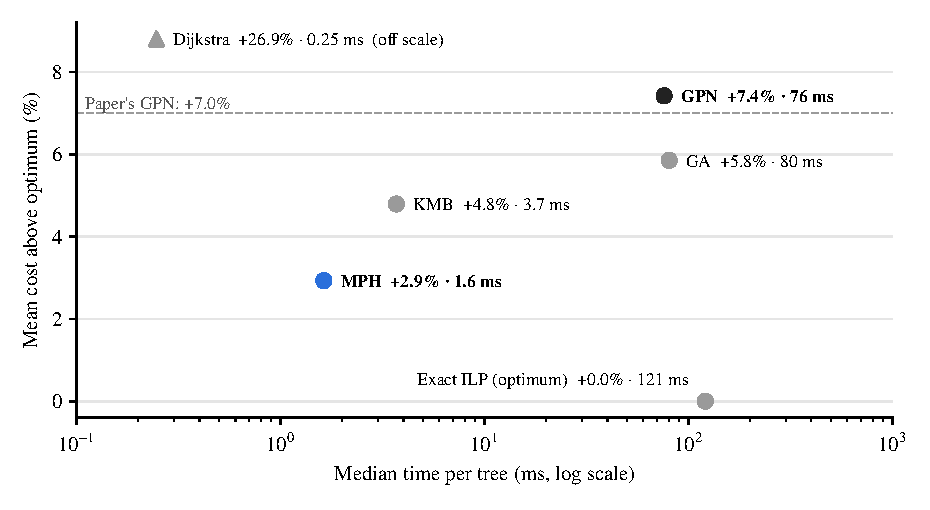
\includegraphics[width=0.75\textwidth]{cost_vs_time_reg50.pdf}
\caption[Cost above optimum vs.\ time per tree (50-node graphs)]{MPH builds cheaper trees than GPN and is about $45\times$ faster (4-regular 50-node graphs, 100 instances; GPN on a T4 GPU at batch size 1, others on CPU). The dashed line marks the paper's reported GPN gap.}
\label{fig:cost_time}
\end{figure}

\noindent Per tree, GPN beats MPH on only about one instance in five (Figure~\ref{fig:hist}). On exact (float64) tree costs, GPN is strictly cheaper on 15--23\% of trees and ties on 7--18\%, so MPH is at least as cheap on 77--85\%. When GPN wins it wins by 2.5--3.6\% of MPH's cost; when it loses it loses by 5.5--7.7\%. Our GA (5.4\% above optimal at 30 nodes) is weaker than the paper's undocumented GA (0.8\%), so it is not presented as the paper's.

\begin{figure}[!htb]
\centering
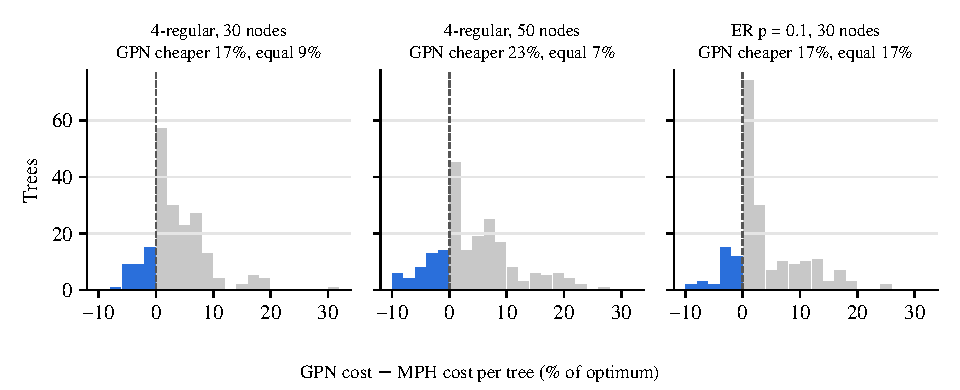
\includegraphics[width=0.95\textwidth]{gpn_minus_mph_hist.pdf}
\caption[Per-tree difference between GPN and MPH costs]{Per-tree GPN cost minus MPH cost, as a percentage of the optimum (2 seeds $\times$ 100 graphs per setting). Blue: GPN cheaper; grey: MPH cheaper or equal.}
\label{fig:hist}
\end{figure}

\noindent Installing the cheaper of the GPN and MPH trees (the safety net with $\varepsilon=0$ and no capacities) lands within 1.6--2.1\% of optimal (Table~\ref{tab:safetynet}), but on static trees it improves on MPH alone by under 1\%.

\begin{table}[!htb]
\caption{Effect of installing the cheaper of the GPN and MPH trees ($\varepsilon=0$, no capacities; ranges span the two seeds)}
\label{tab:safetynet}
\begin{center}
\footnotesize
\setlength{\tabcolsep}{4pt}
\renewcommand{\arraystretch}{1.1}
\begin{tabular}{|c|C{2.3cm}|C{1.5cm}|C{2.0cm}|C{1.9cm}|C{2.0cm}|C{2.0cm}|}
\hline
\textbf{Setting} & \textbf{GPN strictly cheaper} & \textbf{Tie} & \textbf{Combined cost / optimum} & \textbf{Saving vs.\ MPH alone} & \textbf{GPN margin when it wins} & \textbf{GPN margin when it loses} \\
\hline\hline
reg30 & 17\% & 8--10\% & 1.019 & 0.43--0.45\% & 2.5--2.7\% & 5.5--5.6\% \\ \hline
reg50 & 22--23\% & 7\% & 1.021 & 0.78--0.79\% & 3.4--3.6\% & 7.1--7.7\% \\ \hline
gnp30 & 15--19\% & 15--18\% & 1.016--1.017 & 0.48--0.57\% & 3.0--3.2\% & 6.1\% \\
\hline
\end{tabular}
\end{center}
\end{table}

\section{Discussion}\label{sec:r_discussion}
\noindent The public code, once patched, reproduces the paper within 0.004 and is a sound starting point for the encoder of the learned decision policy. The paper, however, misses a strong classical baseline: layered MPH is strictly cheaper than GPN on 66--75\% of instances and far faster. This finding, limited to static trees, has four consequences for the thesis:
\begin{enumerate}
    \item cheaper one-shot trees cannot be the reason to use a GNN; its value must come from the keep / repair / re-plan decision under churn, which the design in Section~\ref{sec:m_policy} already targets;
    \item the safety net bounds cost by a constant factor from layered MPH, not the single-rate $2(1-1/l)$ the proposal claimed, and must show its value on repaired trees;
    \item the main baseline for the repair operators becomes a full MPH re-plan per event, and the threshold policies compared with the learned policy re-plan with MPH;
    \item the risk that the GNN does not beat threshold rules is higher, so the relative weight of the repair operators and fast-failover protection will be agreed with the advisor.
\end{enumerate}
\noindent Only 30--50-node static graphs with 12 users were tested, GPN was timed at batch size 1 with Python overhead, and the layered MPH is our own variant. The next check re-runs the trained model on 100--200-node graphs and Topology Zoo networks, and times batched GPN inference.

\section{Conclusions}\label{sec:c_conclusions}
\noindent The first phase has fixed the research questions and objectives, reviewed the literature and identified the gap, designed the method, surveyed the DoT 5G lab (no 5G MBS, no OpenFlow in the lab switch, a shared lab), and reproduced the base paper within 0.004 of its cost ratio, together with a missing-baseline finding against layered MPH. The remaining work therefore builds the maintenance layer on a verified starting point.

\section{Future Scope}\label{sec:c_future}
\noindent The remaining work builds and evaluates the maintenance layer on the verified starting point:
\begin{enumerate}
    \item Event-driven simulator, cost model and repair operators; first cost-vs-churn results comparing local repair with full re-planning, and a conference paper draft.
    \item Masked keep/repair/re-plan policy with the MPH safety net; ablation against threshold rules.
    \item Ryu module with fast-failover backups and two-phase updates; Tier~2 Mininet measurements of recovery time and switch state.
    \item Tier~3 experiments in the 5G lab with XR headsets and CPEs as receivers.
    \item Thesis writing, open-source release of the controller module and a live demo.
\end{enumerate}
\noindent Lab experiments run on a dedicated VLAN without touching core or RAN settings.


%**************************************************BIBLIOGRAPHY********************************************************
\fancyhead[LE]{\bfseries\small{Bibliography}}
\fancyhead[RO]{\bfseries\small{Bibliography}}
\pdfbookmark[1]{Bibliography}{los}
\addstarredchapter{Bibliography}   % PKM 05/07/08 (For more options refer minitoc.pdf on page 36)
\baselineskip 14pt   %12, 18 and 24
\small
\bibliographystyle{unsrt}
\bibliography{chapters/references/references}

\end{document}
